\lecture{2}{2. September 2025}{Free motion/eigenmotion of SDOF systems}

\exercise{2.1}
We consider the shown system, which is to be analysed as an equivalent single-degree of freedom system (SDOF-system) with the transverse motion of the point mass $m$ as the degree of freedom. It is noted, that the stiffness of the beam (without taking the discrete springs into account) against transverse direction in the free end due to a transverse force acting in this point is $k_{\mathrm{beam}} = \frac{3EI}{L^3}$, where $L$, $I$, and $E$ is the length, area-moment of inertia and the elastic modulus of the beam. Assume, that the beam and the discrete springs are mass-less.

\begin{figure} [ht]
  \centering
  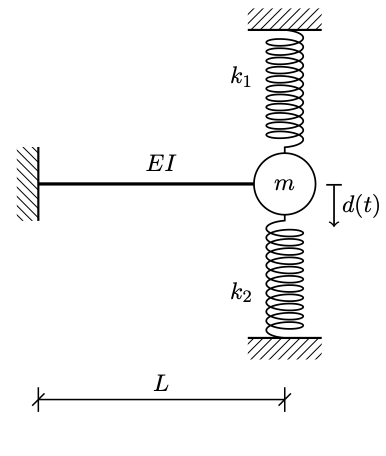
\includegraphics[width=0.35\linewidth]{./figures/f2_1.png}
\end{figure}

\paragraph{a)} Determine (symbolically) the undampened angular eigenfrequency $\omega_u$ of the equivalent SDOF-system.
\bigbreak
The undampened angular eigenfrequency $\omega_u$ is given as:
\[ 
\omega_u = \sqrt{\frac{k}{m}}
.\]
In this case the three springs are connected in parallel and so:
\[ 
  k_{eq} = k_{\mathrm{beam}} + k_1 + k_2 = k_1 + k_2 + \frac{3EI}{L^3}
.\]
And therefore the undampened angular eigenfrequency of the system is
\[ 
  \omega_u = \sqrt{\frac{k_1 + k_2 + \frac{3EI}{L^3}}{m}}
.\]


\paragraph{b)}
It is now noted that (in SI-units) $EI = 100$, $L = \num{1,3}$, $m = \num{0,5}$, $k_1 = k_2 = 25$, $d_0 = \num{0.1}$ and $\dot{d}_0 = 0$. Determine the undampened eigenperiod of the equivalent SDOF-system.
\bigbreak
Note that the connection between frequency as determined in a) and period is:
\[ 
T = \frac{2\pi}{\omega_u} = \frac{2\pi}{\sqrt{\frac{2 \cdot 25 + \frac{300}{\num{1,3}^3}}{\num{0,5} }}} = \qty{0,33}{s} 
.\]


\paragraph{c)}
Determine the maximal speed, that the equivalent SDOF-system experiences in its eigenmotion.
\bigbreak
The displacement $d(t)$ is given as:
\[ 
d(t) = A \cos \left( \omega_u t - \phi \right)
.\]
And the speed $\dot{d}(t)$ can be found simply vie differentiation as
\[ 
\dot{d}(t) = - \omega_u A \sin \left( \omega_u t - \phi \right)
.\]
In its maximum this is
\[ 
\mathrm{max}(\dot{d}(t)) = \omega_u A
.\]
We also know that:
\[ 
A = \sqrt{A_1^2 + A_2^2} = \sqrt{d_0^2 + \frac{\dot{d}_0^2}{\omega_u^2}} = d_0
.\]
Therefore the maximum velocity is:
\[ 
\mathrm{max} \left( \dot{d} (t) \right) = \omega_u A = \sqrt{\frac{k_1 + k_2 + \frac{3EI}{L^3}}{m}} \cdot d_0 = \qty{1,73}{\frac{m}{s}}
.\]



\exercise{2.2}
With reference to the following harmonic response choose the correct starting conditions.

\begin{figure} [ht]
  \centering
  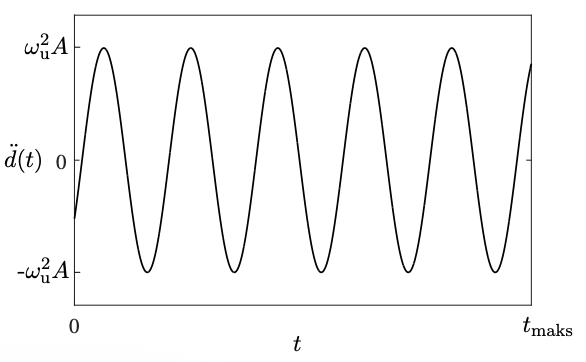
\includegraphics[width=0.35\linewidth]{./figures/f2_2.png}
\end{figure}

\begin{enumerate}
  \item $d_0 < 0 \wedge \dot{d}_0 = 0$
  \item $d_0 > 0 \wedge \dot{d}_0 = 0$
  \item $d_0 < 0 \wedge \dot{d}_0 > 0$
  \item $d_0 > 0 \wedge \dot{d}_0 < 0$
  \item $d_0 = 0 \wedge \dot{d}_0 > 0$
  \item $d_0 = 0 \wedge \dot{d}_0 < 0$
\end{enumerate}
\bigbreak
The plot looks to be showing sinusoidal acceleration. In the initial case the acceleration is negative, this means that the speed here is necessarily also negative, a negative speed means that the initial displacement must have been positive, hence the correct answer is 4


\exercise{2.3}
We consider the shown system, which is to be analysed as an equivalent SDOF-system, wherein the degree of freedom is horizontal movement of the horizontal beam. It is noted that the horizontal beam has mass $m$ and is assumed to be infinitely stiff, whilst the two vertical beams are assumed massless and with stiffness $k$.

\begin{figure} [ht]
  \centering
  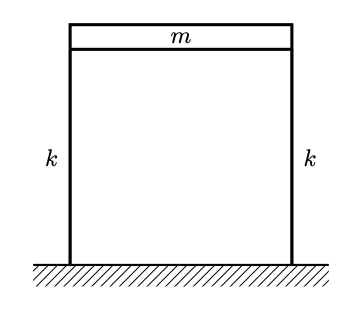
\includegraphics[width=0.5\linewidth]{./figures/f2_3.png}
\end{figure}

\paragraph{a)}
Determine (symbolically) what the undampened angular eigenfrequency $\omega_u$ of the equivalent SDOF-system is.
\bigbreak
The two beams are connected in parallel, hence:
\[ 
k_{eq} = 2k \implies \omega_u = \sqrt{\frac{2k}{m}}
.\]


\paragraph{b)}
It is noted that (in SI-units) $m = 3$, $k = 30$, $d_0 = -\num{0,1}$, and $\dot{d}_0 = \num{0,2}$. Determine the initial acceleration of the equivalent SDOF-system
\bigbreak
From Newton's second law we get:
\[ 
m \ddot{d}(t) + k d(t) = 0 \implies m \ddot{d}_0 + k_{eq} d_0 = 0
.\]
And now we can solve for $\ddot{d}_0$ as:
\[ 
\ddot{d}_0 = \frac{- k_{eq} d_0}{m} = \frac{- 60 \cdot (- \num{0,1})}{3} = \qty{2}{\frac{m}{s}} 
.\]

